\documentclass[a4 paper, 12pt]{report}
\usepackage{hyperref}
\usepackage{apacite}
\usepackage{amssymb,dsfont,amsthm,amsmath,makeidx,verbatim,latexsym,amsfonts,mathrsfs}
%\usepackage[latin9]{inputenc}
%\usepackage[utf8]{inputenc}
%\usepackage[T1]{fontenc}
\usepackage{titlesec}
\setcounter{secnumdepth}{4}
\usepackage[authoryear]{natbib}
\usepackage{hyperref}
\usepackage{tikz-cd}
\usepackage{graphicx}
\usepackage[none]{hyphenat}
\usepackage{tabularx}
\usepackage{lmodern}
\usepackage[tikz]{bclogo}
\usepackage{cancel}
\usepackage{framed, color}
%\usepackage[standard, amsmath, thmmarks]{ntheorem}
\usepackage{cleveref}
%\usepackage{fourier}
\usepackage{mathtools}

\usepackage[english]{babel}
\addto{\captionsenglish}{%
  \renewcommand{\bibname}{REFERENCES}
	%\renewcommand{\tableofcontents}{Table of Contents}
}


\DeclareMathAlphabet{\mathpzc}{OT1}{pzc}{m}{it}
\newcommand*\rfrac[2]{{}^{#1}\!/_{#2}}

\hfuzz5pt
\theoremstyle{plain}
\newtheorem{theorem}{\textbf{Theorem}}[section]
\newtheorem{lemma}[theorem]{\textbf{Lemma}}
\newtheorem{proposition}[theorem]{\textbf{Proposition}}
\newtheorem{corollary}[theorem]{\textbf{Corollary}}
\newtheorem{claim}[theorem]{\textbf{Claim}}
\newtheorem{addendum}[theorem]{\textbf{Addendum}}
\newtheorem{definition}[theorem]{\textbf{Definition}}
\newtheorem{remark}[theorem]{\textbf{Remark}}
\newtheorem{example}[theorem]{\textbf{Example}}
\newtheorem{conjecture}[theorem]{\textbf{Conjecture}}
\newtheorem{notation}[theorem]{\textbf{Notation}}
\renewcommand{\baselinestretch}{1.50} % for the line spacing.
%\newcommand*\rfrac[2]{{}^{#1}\!/_{#2}}
\begin{document}
\section*{L$\ddot{\mbox{o}}$sung}
\subsection*{Teilaufgabe Teil A 1a (2 BE)}
Die Abbildung zeigt ein gerades Prisma $A ~B~ C~ D~ E~ F$ mit $A(0|0|0), B(8|0|0), C(0|8|0)$ und $D(0|0|4).$
\begin{figure}[h]
	\centering
		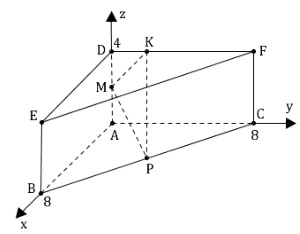
\includegraphics{image1.jpg}
	\label{fig:image1}
\end{figure}$$$$
Bestimmen Sie den Abstand der Eckpunkte B und F.
\subsection*{\underline{L$\ddot{\mbox{o}}$sung zu Teilaufgabe Teil A 1a}}
\textbf{L$\ddot{\mbox{a}}$nge eines Vektors}
\begin{figure}[h]
	\centering
		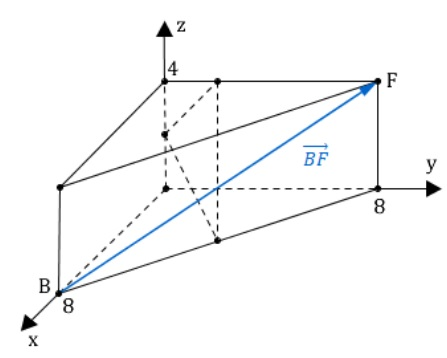
\includegraphics[width=0.40\textwidth]{image2.jpg}
	\label{fig:image2}
\end{figure}
\newpage
$B(8|0|0), F(0|8|4)$
$$
\stackrel{\longrightarrow}{BF} = \stackrel{\longrightarrow}{F} - \stackrel{\longrightarrow}{B} = 
\begin{pmatrix}
&0&\\
&8&\\
&4&
\end{pmatrix}
-
\begin{pmatrix}
&8&\\
&0&\\
&0&
\end{pmatrix}
= 
\begin{pmatrix}
&-8&\\
&8&\\
&4&
\end{pmatrix}
$$
$$
\overline{BF} = |\stackrel{\longrightarrow}{BF}| = \left|
\begin{pmatrix}
&-8&\\
&8&\\
&4&
\end{pmatrix}
\right| = \sqrt{(-8)^2+8^2+4^2}=12
$$
\textbf{\large{Teilaufgabe Teil A 1b (3 BE)}}\\
Die Punkte M und P sind die Mittelpunkte der Kanten $[AD]$ bzw. $[B C]$.\\
Der Punkt $K (0|y K |4)$ liegt auf der Kante [DF]. Bestimmen Sie y K so, dass das Dreieck $K~M~P$ in $M$ rechtwinklig ist.
\subsection*{\underline{L$\ddot{\mbox{o}}$sung zu Teilaufgabe Teil A 1b}}
\textbf{Mittelpunkt einer Strecke}
\begin{figure}[h]
	\centering
		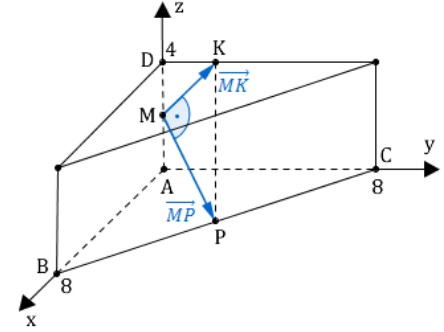
\includegraphics[width=0.70\textwidth]{image3.jpg}
	\label{fig:image3}
\end{figure}
\newpage
$A(0|0|0), D(0|0|4)$\\
$B(8|0|0), C(0|8|0)$
\begin{align*}
\stackrel{\longrightarrow}{M}& = \frac{1}{2}\cdot \bigg[\stackrel{\longrightarrow}{A}+\stackrel{\longrightarrow}{D}\bigg] = \frac{1}{2}\cdot\left[
\begin{pmatrix}
&0&\\&0&\\&0&
\end{pmatrix}
+
\begin{pmatrix}
&0&\\&0&\\&4&
\end{pmatrix}
\right]
 = \frac{1}{2}
\begin{pmatrix}
&0&\\&0&\\&4&
\end{pmatrix}
= 
\begin{pmatrix}
&0&\\&0&\\&2&
\end{pmatrix}\\
&\Longrightarrow M(0|0|2)
\end{align*}



\begin{align*}
\stackrel{\longrightarrow}{P}& = \frac{1}{2}\cdot \bigg[\stackrel{\longrightarrow}{B}+\stackrel{\longrightarrow}{C}\bigg] = \frac{1}{2}\cdot\left[
\begin{pmatrix}
&8&\\&0&\\&0&
\end{pmatrix}
+
\begin{pmatrix}
&0&\\&8&\\&0&
\end{pmatrix}
\right]
 = \frac{1}{2}
\begin{pmatrix}
&8&\\&8&\\&0&
\end{pmatrix}
= 
\begin{pmatrix}
&4&\\&4&\\&0&
\end{pmatrix}\\
&\Longrightarrow P(4|4|0)
\end{align*}
\textbf{Skalarprodukt}
\begin{align*}
\stackrel{\longrightarrow}{MK} &= \stackrel{\longrightarrow}{K}-\stackrel{\longrightarrow}{M} = 
\begin{pmatrix}
&0&\\
&yk&\\
&4&
\end{pmatrix}
-
\begin{pmatrix}
&0&\\
&0&\\
&2&
\end{pmatrix}
=
\begin{pmatrix}
&0&\\
&yk&\\
&2&
\end{pmatrix}\\
\stackrel{\longrightarrow}{MP}& = \stackrel{\longrightarrow}{P}-\stackrel{\longrightarrow}{M} = \begin{pmatrix}&4&\\&4&\\&0&\end{pmatrix}-\begin{pmatrix}&0&\\&0&\\&2&\end{pmatrix} =  \begin{pmatrix}&4&\\&4&\\&-2&\end{pmatrix}\\
\stackrel{\longrightarrow}{MK}\circ \stackrel{\longrightarrow}{MP}& = 
\begin{pmatrix}
&0&\\
&yk&\\
&2&
\end{pmatrix}
\circ
\begin{pmatrix}
&4&\\&4&\\&-2&
\end{pmatrix} = 0+4yk-4
\end{align*}
Es soll gelten: $\stackrel{\longrightarrow}{MK}\circ \stackrel{\longrightarrow}{MP} = 0$\\
$4yk-4 = 0$\\
$\Longrightarrow~~~~yk = 1$

\subsection*{Teilaufgabe Teil A 2a (1 BE)}
Gegeben ist die Ebene E : $3x_2+4x_3 = 5$.\\
Beschreiben Sie die besondere Lage von E im Koordinatensystem.
\subsection*{\underline{L$\ddot{\mbox{o}}$sung zu Teilaufgabe Teil A 2a}}
\textbf{\large Besondere Lage im Koordinatensystem}\\
$\stackrel{\longrightarrow}{n_E} = 
\begin{pmatrix}
&0&\\
&3&\\
&4&
\end{pmatrix}
$\\
Die Ebene E ist parallel zur $x_1$-Achse, da die $x_1$-Koordinate des Normalenvektors Null ist.
\subsection*{Teilaufgabe Teil A 2b (4 BE)}
Untersuchen Sie rechnerisch, ob die Kugel mit Mittelpunkt $Z(1|6|3)$ und Radius $7$ die
Ebene E schneidet.
\newpage
\subsection*{L$\ddot{\mbox{o}}$sung zu Teilaufgabe Teil A 2b}
%\newpage
\textbf{Abstand Punkt - Ebene}
%\newpage
\begin{figure}[h]
	\centering
		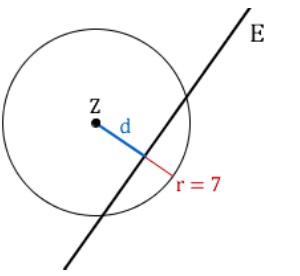
\includegraphics[width=0.50\textwidth]{image4.jpg}
	\label{fig:image4}
\end{figure}
%\newpage
$$$$
$Z(1|6|3)$\\
$E: 3x_2+4x_3 = 5$\\
$\stackrel{\longrightarrow}{n_E} = \begin{pmatrix}
&0&\\
&3&\\
&4&
\end{pmatrix}~~~$Normalenvektor der Ebene\\
Betrag des Normalenvektors bestimmen:
$$
|\stackrel{\longrightarrow}{n_E}| = \left|\begin{pmatrix}
&0&\\
&3&\\
&4&
\end{pmatrix}
\right| = \sqrt{0+3^2+4^2} = 5
$$
Hesse-Normalenform $E^{HNF}$ der Ebene aufstellen:\\
$E^{HNF}:\frac{1}{5}(3x_2+4x_3-5) = 0$\\
Abstand bestimmen:
$$
d = d(Z,E) = \bigg|\frac{1}{5}(3\cdot 6+ 4\cdot 3-5)\bigg| = 5<r(=7)
$$
Der Abstand des Mittelpunktes Z zur Ebene E ist kleiner als der Radius r der Kugel, also
schneiden sich Kugel und Ebene.
\subsection*{Teilaufgabe Teil B a (3 BE)}
In einem kartesischen Koordinatensystem legen die Punkte $A(4|0|0), B(0|4|0)$ und $C(0|0|4)$ das Dreieck AB C fest, das in der Ebene $E : x_1 + x_2 + x_3 = 4$ liegt.\\
Bestimmen Sie den Fl$\ddot{\mbox{a}}$cheninhalt des Dreiecks $A~B~C$.
\subsection*{\underline{L$\ddot{\mbox{o}}$sung zu Teilaufgabe Teil B a}}
\textbf{\large Fl$\ddot{\mbox{a}}$cheninhalt eines Dreiecks}
\begin{align*}
A(4|0|0),& B(0|4|0) \mbox{  und  } C(0|0|4)\\
\stackrel{\longrightarrow}{AB}& = \stackrel{\longrightarrow}{B}-\stackrel{\longrightarrow}{A} = 
\begin{pmatrix}
&0&\\
&4&\\
&0&\\
\end{pmatrix}
-
\begin{pmatrix}
&4&\\
&0&\\
&0&\\
\end{pmatrix}
=
\begin{pmatrix}
&-4&\\
&4&\\
&0&\\
\end{pmatrix}\\
\stackrel{\longrightarrow}{AC}& = \stackrel{\longrightarrow}{C}-\stackrel{\longrightarrow}{A} = 
\begin{pmatrix}
&0&\\
&0&\\
&4&\\
\end{pmatrix}
-
\begin{pmatrix}
&4&\\
&0&\\
&0&\\
\end{pmatrix}
=
\begin{pmatrix}
&-4&\\
&0&\\
&4&\\
\end{pmatrix}
\end{align*}

Fl$\ddot{\mbox{a}}$cheninhalt des Dreiecks $A~B~C:$
$$
A_{ABC} = \frac{1}{2}\cdot\left|
\begin{pmatrix}
&-4&\\
&4&\\
&0&
\end{pmatrix}
\times
\begin{pmatrix}
&-4&\\
&0&\\
&4&
\end{pmatrix}
\right|
$$
$$
A_{ABC} = \frac{1}{2}\cdot
\left|
\begin{pmatrix}
&16&\\
&16&\\
&16&
\end{pmatrix}
\right|
 = 
\frac{1}{2}
\cdot
\left|16\cdot
\begin{pmatrix}
&1&\\
&1&\\
&1&
\end{pmatrix}
\right|
=\frac{1}{2}\cdot 16\cdot
\left|
\begin{pmatrix}
&1&\\
&1&\\
&1&
\end{pmatrix}
\right|
$$
$$
A_{ABC} = 8\cdot\sqrt{1^2+1^2+1^2} = 8\sqrt{3}
$$
\subsection*{Teilaufgabe Teil B b (5 BE)}

Das Dreieck $A~B~C$ stellt modellhaft einen Spiegel dar. Der Punkt $P(2|2|3)$ gibt im Modell die Position einer Lichtquelle an, von der ein Lichtstrahl ausgeht. Die Richtung dieses
Lichtstrahls wird im Modell durch den Vektor $\stackrel{\longrightarrow}{v} = \begin{pmatrix}
&-1&\\
&-1&\\
&-4&\\
\end{pmatrix}
$ ~~beschrieben.

Geben Sie eine Gleichung der Geraden g an, entlang derer der Lichtstrahl im Modell
verl$\ddot{\mbox{a}}$uft. Bestimmen Sie die Koordinaten des Punkts R, in dem g die Ebene E schneidet,
und begr$\ddot{\mbox{u}}$nden Sie, dass der Lichtstrahl auf dem dreieckigen Spiegel auftrifft.\\
( zur Kontrolle: $R(1,5|1,5|1)$)
\subsection*{\underline{L$\ddot{\mbox{o}}$sung zu Teilaufgabe Teil B b}}
\textbf{\large Geradengleichung aufstellen}
$$
g:\stackrel{\longrightarrow}{X} = \underbrace{\begin{pmatrix}&2&\\&2&\\&3&\end{pmatrix}}_{\stackrel{\longrightarrow}{P}}
+\lambda\cdot \underbrace{\begin{pmatrix}&-1&\\&-1&\\&-4&\end{pmatrix}}_{\stackrel{\longrightarrow}{v}}
$$
\textbf{Schnitt Ebene und Gerade}\\
$E:x_1+x_2+x_3 = 4$\\
Ebene $E$ und Gerade $g$ schneiden: $E\cap g$.
\begin{align*}
E\cap g: (2-\lambda)+&(2-\lambda)+(3-4\lambda)& = 4\\
&7-6\lambda& = 4\\
&-6\lambda& = -3\\
&\lambda& = \frac{1}{2}
\end{align*}
$$
\stackrel{\longrightarrow}{R} = 
\begin{pmatrix}
&2&\\
&2&\\
&3&\\
\end{pmatrix}
+\frac{1}{2}\cdot
\begin{pmatrix}
&-1&\\
&-1&\\
&-1&\\
\end{pmatrix}
=
\begin{pmatrix}
&1,5&\\
&1,5&\\
&1&\\
\end{pmatrix}
~~~\Longrightarrow~~ R(1,5|1,5|1)
$$

Begr$\ddot{\mbox{u}}$ndung:\\
Alle Koordinaten von R sind positiv.



\end{document}